\documentclass[12pt,english]{amsart}
\usepackage[utf8]{inputenc}
%\usepackage[margin=0.5in]{geometry}
\usepackage[a4paper, margin=2cm]{geometry}
\linespread{1.5}

%\usepackage{fontspec}
%\setmainfont{Times New Roman}
\usepackage{mathptmx}

\usepackage{graphicx}
\usepackage{wrapfig}
\usepackage{lscape}
\usepackage{rotating}
\usepackage{epstopdf}

\usepackage{verbatim}
\usepackage{url}
\usepackage{xspace}
%\usepackage{wrapfig}

\usepackage{listings}
\usepackage{color}
    \definecolor{light}{gray}{0.97}
    \definecolor{dark}{gray}{0.30}
\lstset{
%columns=fullflexible,
%basicstyle=\ttfamily,
escapeinside={||},
    %mathescape=true,
    language=C, % choose the language of the code
    basicstyle=\fontfamily{pcr}\selectfont\scriptsize\color{black},
    keywordstyle=\color{black}\bfseries, % style for keywords
    numbers=none, % where to put the line-numbers
    numberstyle=\tiny, % the size of the fonts that are used for the line-numbers
    backgroundcolor=\color{light},
    showspaces=false, % show spaces adding particular underscores
    showstringspaces=false, % underline spaces within strings
    showtabs=false, % show tabs within strings adding particular underscores
    %frame=single, % adds a frame around the code
    tabsize=2, % sets default tabsize to 2 spaces
    %rulesepcolor=\color{gray}
    captionpos=b, % sets the caption-position to bottom
    breaklines=false, % sets automatic line breaking
    %breakatwhitespace=false,
    numbersep=2em,
    % C was used in the blocksworld example to refer to block C and nowhere else
    emph={par,or,hor,do,end,loop,code,await,pause,emit,input,event,call,with,%
          var,and,then,else,return,pure,deterministic,nohold,finalize,%
          class, every, FOREVER, this, spawn, in, pool, watching, until, 
          interface, each, abort, when, signal, PROC, CHAN, SIGNAL, PAR, not,
          bool, tag, escape, traverse,implementation,output,true,false,
          native,@const,@pure,@safe,define,public,private,none},
    emphstyle={\bfseries},
    commentstyle=\color{dark}\scriptsize,
    %xleftmargin=20pt,
    %xrightmargin=20pt,
    framesep=20pt,
    %upquote=true,
    %aboveskip={1.5\baselineskip},
}

%\newcommand{\CEU}{\textsc{C\'{e}u}\xspace}
\newcommand{\code}[1] {{\small{\texttt{#1}}}}

\usepackage{enumitem}
\setlist{nolistsep}

% Auto-Standby
\title{Eficiência Energética para Software IoT em Larga Escala}

%\author{Anonymous Author}

\begin{document}

\date{}
\maketitle

\vspace{-1cm}
\begin{comment}
\abstract{
TODO
}
\end{comment}

%\newpage
\section{Narrativa Profissional}

Trabalho no campo de \emph{Linguagens de Programação} com o foco em 
\emph{Sistemas Reativos de Tempo Real}.
Sistemas reativos interagem continuamente com o mundo externo através de
sensores e atuadores (e.g., botões, LEDs e motores).
Quando essas interações têm que cumprir prazos estritos, o sistema é dito de
\emph{tempo real}.
A maioria das aplicações do dia-a-dia, tais como suítes de escritório e jogos
eletrônicos são reativas mas bastante tolerante a atrasos.
Em contraste, sistemas embarcados de tempo real, tais como aplicações médicas,
sistemas de aviação, e dispositivos de IoT, devem cumprir prazos mais estritos.

No início do meu Mestrado, me juntei ao grupo de desenvolvimento do
\emph{Ginga}, o padrão de software do Sistema Digital da TV
Brasileira~\cite{ncl.abnt}, que também se tornou um padrão
ITU/UN~\cite{ncl.itu}.
Durante esse período, trabalhei numa integração não intrusiva entre as duas
linguagens padronizadas NCL e Lua através de uma interface de programação
reativa.
O resultado desse trabalho foi publicado no \emph{ACM DocEng} de 2009.
Também escrevi o capítulo sobre desenvolvimento em Lua e NCL do livro de
referência do Ginga.

Em 2009, iniciei o programa de Doutorado com o objetivo de projetar uma nova
linguagem reativa desde o início, agora direcionada a sistemas embarcados com
recursos restritos.
Por um lado, essas plataformas são tipicamente seis ordem de magnitude menos
poderosas que computadores tradicionais em termos de memória e processamento.
Por outro lado, aplicações embarcadas necessitam de mais confiabilidade para
operar sem a intervenção humana por longos períodos de tempo.
Além disso, um subconjunto significativo de sistemas embarcados é implantado
em locais sem linhas de energia e devem funcionar com baterias.
Sendo assim, uma linguagem de programação direcionada a sistemas embarcados
restritos deve ser pequena, confiável e eficiente energeticamente.
Ao final de 2012, me tornei bolsista da \emph{SAAB Aerospace} para um período
de seis meses de pesquisa.
Juntei-me a um grupo de pesquisa em uma universidade da Suécia e reescrevemos
drivers e protocolos de rede de qualidade industrial.
Conseguimos uma redução considerável no tamanho do código fonte, com uso
similar de recursos em comparação com C.
Em 2013, publicamos um artigo com esses resultados no \emph{ACM SenSys}.

Após me graduar, contribuí com o projeto \emph{Cidades Inteligentes}, que
envolve 20 universidade e busca construir uma infraestrutura de IoT.
%
Em 2015, em cooperação com um aluno de Doutorado, publicamos um artigo no
\emph{ACM TOSN}, mostrando que podemos reprogramar dispositivos embarcados
remotamente usando menos energia do que o estado da arte.
%
Durante o mesmo período, publiquei um artigo no
\emph{Int'l Conference on Modularity}
propondo uma nova abstração de concorrência que gera programas mais modulares.
%
Também fui convidado a apresenta minha linguagem de pesquisa em um encontro
anual do \emph{Working Group on Language Design} grupo afiliado com a IFIP da
UNESCO.

Atualmente, como professor associado em uma universidade brasileira, continuo
a investigar como o projeto de linguagens pode afetar o desenvolvimento de
aplicações reativas.
Durante os últimos 4 anos, publiquei ou atuei no comitê do
\emph{Int'l Workshop on Reactive Languages}.
Em 2017, publiquei um artigo consolidando o projeto da minha linguagem de
pesquisa no \emph{ACM TECS}.

\section{Divulgação Científica: O Papel do Software IoT na Eficiência Energética}

De acordo com a Agência Internacional de Energia (IEA)~\cite{iea.data},
existiam em torno de 14 bilhões de dispositivos conectados tradicionais em 2013
(e.g., telefones TVs inteligentes).
Esse número deve crescer para 50 bilhões em 2020 com a proliferação de
dispositivos IoT (e.g., lâmpadas inteligentes e tecnologia vestível).
%
Dispositivos IoT e tradicionais já superam o número de pessoas no planeta por
um fator de dois, e o tráfego de dados é esperado crescer a uma taxa
exponencial nos próximos anos.
%
No entanto, a maior parte da energia desses aparelhos é consumida quando eles
estão em \emph{standby} (\emph{modo em espera}).
%
A emissão anual de $CO_2$ relacionada a standby é equivalente a de 1 milhão de
carros.
%
A projeção de crescimento de IoT, juntamente com o efeito surpreendente dos
efeitos de consumo de standby, fizeram com que a eficiência de standby para
dispositivos conectados fosse um dos seis pilares do \emph{Plano de Ação para
Eficiência Energética} do G20%
\footnote{G20's Energy Efficiency Action Plan: \url{https://www.iea-4e.org/projects/g20}}.

Outras organizações também reportaram sobre a importância da economia de
energia em dispositivos conectados.
%
Para o \emph{Internet Engineering Task Force (IETF)}, ``o gerenciamento
energético está se tornando um requisito adicional para redes devido a diversos
fatores que incluem o aumento dos custos de energia, o impacto ecológico para
a operação das redes, e a regulação de energia''~\cite{ietf.eman}.
%
Para o \emph{American Council for an Energy-Efficient Economy (ACEEE)},
``o potencial para a nova eficiência energética permanece enorme, (...) devemos
considerar uma abordagem sistêmica para escalar a eficiência energética.
(...) a eficiência inteligente é adaptativa, antecipatória, e
conectada''~\cite{aceee.1}.

Considerando iniciativas concretas, o grupo de trabalho
\emph{Electronic Devices and Networks} da IEA foca especificamente na questão
do standby em dispositivos conectados%
\footnote{EDNA initiative: \url{https://edna.iea-4e.org/}}.
A iniciativa da ACEEE em \emph{Intelligent Efficiency} promove uma abordagem
sistemática para otimizar o comportamento cooperativo de dispositivos de modo
a buscar ganhos de energia como um todo.
Ambos as abordagens, por dispositivo e sistêmica, envolvem soluções de
software, dado que a economia de energia é uma política dinâmica que depende
das demandas das aplicações e níveis de baterias em um determinados momentos.
%
Também existem padrões de baixo consume de energia para a infraestrutura de IoT
com diferentes demandas de alcance, velocidade e distribuição
física~\cite{iot.energy.2}.
Como exemplo, o \emph{Bluetooth Low-Energy (BLE)} é um substituto para o padrão
Bluetooth clássico e é projetado para baixas velocidades em redes pessoais
(PANs).
O \emph{6LoWPAN} adapta o padrão IPv6 para baixo consumo e em dispositivos de
processamento limitado.
%
Essas tecnologias permitem transmissões mais eficientes, suportam topologias
flexíveis e reduzem o tráfego consideravelmente.
Elas também possibilitam o uso de modos de standby mínimos.
%
No entanto, essas tecnologias exigem o uso de software para controlar os modos
ativos e de standby de maneira a construir uma IoT eficiente em termos de
energia.

%\newpage
\section{Resumo Científico}

O uso efetivo de standby terá papel fundamental na eficiência energética para
os 50 bilhões de dispositivos IoT esperados até 2020~\cite{iea.data}.
%
Este projeto de pesquisa visa endereçar os desafios de software, conforme
determinados pela IEA, em direção a uma IoT eficiente em termos de
energia~\cite{iea.data}:
    garantir que os dispositivos adotem os níveis mais econômicos possíveis de
    standby, e que os dispositivos permaneçam o maior período possível em
    standby.

Tendo em vista a escala projetada para a IoT e o papel do modo standby para a
eficiência energética, este projeto de pesquisa tem os seguintes objetivos:

\begin{enumerate}
    \item Endereçar a eficiência energética com o uso criterioso de standby.
    \item Focar em arquiteturas embarcadas restritas que formam a IoT.
    \item Prover mecanismos de standby no nível de linguagens de programação para
          escalar para todas as aplicações.
    \item Suportar mecanismos de standby transparentes e não intrusivos para
          reduzir as barreiras de adoção.
\end{enumerate}

Muitas linguagens, extensões e sistemas operacionais direcionados à energia
foram propostos recentemente.
%
Algumas propostas ajustam a QoS (qualidade de serviço) para reduzir o consumo~\cite{os.ecosystem,lang.green,lang.enerj,lang.greenweb}.
%
Outras propostas oferecem mecanismos para trocar o comportamento dependendo das
demandas e níveis de bateria da aplicação~\cite{lang.eon,lang.energytypes,lang.gradual,lang.ent}.
%
Nenhuma dessas iniciativas tira vantagem de modos de standby quando ociosas,
mas somente adaptam ou eliminam computações quando em modo ativo (não
satisfazendo o objetivo 1).

Tenho trabalhado no projeto de uma nova linguagem de programação reativa para
sistemas embarcados restritos pelos últimos 8 anos.
%
A linguagem é baseada no modelo de concorrência síncrono, que troca poder por
confiabilidade e possui um modelo de tempo mais simples que cobre a maioria dos
requisitos de aplicações IoT.
%
Nesse modelo, todas as reações ao mundo externo são computadas em tempo finito,
garantindo que as aplicações sempre chegam a um estado ocioso que é suscetível
ao modo standby.
%
Esperamos que aplicações existentes que não sejam cientes sobre o consumo de
energia irão beneficiar-se de economias na ordem de 50\% baseado nas
estimativas da IEA (considerando as tecnologias atuais de
standby~\cite{iea.data}) e também em trabalhos em ciência transparente de
energia~\cite{wsn.tos.2}.

\section{Projeto Científico}

\subsection{Primeiro Ano}
\label{sec.first}

Necessitaremos de um orçamento de R\$70k:
R\$60k para suporte a três estudantes, R\$5k para equipamentos, e
R\$5k para publicações e custos de viagem.

\subsubsection{Infraestrutura de Hardware para IoT}

Usaremos Arduinos~\cite{arduino} como a principal plataforma de hardware para
IoT.
A maioria dos Arduinos é baseado em microcontroladores de baixo consumo da
Atmel, tais como o \emph{ATmega328p}~\cite{arduino.atmega328p}, suportando
seis modos standby que podem reduzir o consumo para níveis baixíssimos.

No ambiente acadêmica, existe bastante pesquisa com o uso de Arduinos no
contexto de IoT~\cite{arduino.infra,arduino.health,arduino.home,arduino.energy}.
A popularidade do Arduino fará com que a nossa pesquisa seja mais acessível e
reproduzível para outros grupos.
Em educação, muitos cursos em universidades usam o Arduino~\cite{arduino.edu.1,arduino.edu.2,arduino.edu.3,arduino.edu.4}.
Nós temos usado o Arduino em um curso de graduação pelos últimos 3 anos, o que
permitirá avaliar os resultados com programadores de sistemas embarcados menos
experientes.
Na comunidade hobista, há uma abundância de software publicamente disponível
que poderemos adaptar para a nossa linguagem e avaliar os ganhos de eficiência.

\subsubsection{Infraestrutura de Software para IoT}
\label{sec.method.software}

A maneira mais típica em Arduino de interagir com o mundo externo é através de
\emph{polling}, que amostra um periférico externo para detectar mudanças de
estado.
Polling gasta ciclos de CPU e previne que o dispositivo entre em modo standby.
No Arduino, mesmo funcionalidades básicas, tais como temporizadores,
conversores A/D, e SPI, usam ciclos de polling que gastam energia em modo
ativo.

De modo a prover standby automático, as aplicações deve ser inteiramente
reativas a eventos.
%
Recentemente, adicionamos suporte a rotinas de interrupção (ISRs) como um
conceito primitivo na nossa linguagem, o que permitirá reconstruir a
infraestrutura de software IoT com ciência ao modo standby desde sua base.
%
Esse processo consistirá primordialmente de reescrever device drivers, que são
os pedaços de software que interagem diretamente com o hardware.
%
Essa abordagem não irá afetar a maneira como as aplicações são escritas em
níveis mais abstratos, que permanecerá similar às aplicações em Arduino.
No entanto, em vez de gastar ciclos da CPU em espera ativa, as aplicações
entrarão no modo de standby mais profundo possível em quanto estiverem ociosas.

\subsubsection{Aplicações IoT}
\label{sec.method.apps}

De modo a avaliar os ganhos de energia com a infraestrutura proposta,
precisaremos avaliar o consumo em aplicações realistas.
%
A comunidade do Arduino tem uma abundância de projetos open-source que podem
ser reescritos na nossa linguagem para tirar proveito do modo de standby
transparente.
%
Então, poderemos comparar as versões originais e reescritas em termos de
consumo para tirar conclusões sobre a efetividade do modo de standby
transparente.
%
Os cenários mais realistas de IoT usam comunicação por rádio extensivamente.
%
Nesse contexto, iremos avaliar desde protocolos ad-hoc simples até protocolos
mais complexos com ciência energética para ver até que extensão nossa proposta
contribuiria efetivamente em economias de energia.
%
No longo prazo, esperamos mostrar o valor para desenvolvedores reescreverem
suas aplicações na nossa linguagem para tirar proveito dos modos de standby
automáticos.
%
Nessa direção, avaliaremos o tempo tomado para reescrever as aplicações e os
ganhos reais de eficiência energética.

\subsubsection{\textbf{Contribuições Esperadas}}

O vocabulário dedicado a eventos oferecido pela linguagem aumenta o nível de
abstração dos programas para um nível mais próximo do domínio de IoT, provendo
mais segurança e expressividade para programadores.
Até onde sabemos, suporte para ISRs no nível de linguagem ainda não foi
tentado anteriormente.

Nossa proposta visa fazer com que todas as aplicações estejam sujeitas a modos
de standby transparentemente.
Sendo parte da infraestrutura de software, somente device drivers necessitarão
de gerenciamento explícito de energia, e todas as aplicações construídas sobre
eles se beneficiarão de eficiência energética automaticamente.

Nossa linguagem é um projeto de 8 anos e tem uma implementação open-source
madura que está disponível publicamente para downloads.
Com a proposta de adaptação ao contexto de eficiência energética para IoT, a
linguagem pode se tornar uma alternativa prática ao Arduino no curto prazo.

\subsection{Os Três Anos Seguintes}

\subsubsection{Ciência de Energia Sistemática}
\label{sec.method.systematic}

Ciência de energia sistemática considera a rede IoT como um todo, com
dispositivos cooperando para maximizar a eficiência de energia globalmente.
%
Nesse contexto, \emph{computação adaptativa}~\cite{adaptive} é a capacidade
da IoT se adaptar dinamicamente ao consumo de energia, baseando-se na demanda
das aplicações e níveis de bateria durante sua execução.
%
Fundamentalmente, o objetivo ainda é o de que cada dispositivo maximize o tempo
ocioso para ser mais suscetível a modos de standby.
Dessa forma, a pesquisa do primeiro ano é um pré-requisito para essa fase.
%
Nós continuaremos a investigar como mecanismos de linguagens podem propiciar
mais eficiência energética, mas agora em um contexto de computação adaptativa.

O método científico para energia sistemática será similar ao adotado para a
abordagem por dispositivo (conforme discutido na Seção~\ref{sec.method.apps}):
pegar protocolos e aplicações IoT cientes de energia e reescrevê-las usando
mecanismos não intrusivos, e usar os mesmo critérios de avaliação (i.e., tempo
de reescrita, estética do código, e consumo de energia).

\subsubsection{Arquiteturas e Aplicações de IoT Complexas}
\label{sec.method.complex}

A IoT também consiste de dispositivos mais tradicionais, tais como roteadores,
servidores, e smartphones.
%
Em 2016, existiam 3.9 bilhões de assinaturas telefônicas globalmente, e esse
número de alcançar 6.8 bilhões em 2022~\cite{ericsson.mobility}.

Smartphones têm restrições similares de consumo de bateria e também podem tirar
proveito das técnicas propostas para sistemas embarcados restritos.
%
De modo a transpor a barreira de dispositivos restritos para smartphones para a
IoT, percorreremos um caminho similar ao apresentado na Seção~\ref{sec.first}:
%
\begin{description}
\item[Infraestrutura de Hardware]
Usaremos o BeagleBone Black~\cite{bbb.manual}, que compartilha objetivos
similares ao do Arduino, provendo uma plataforma barata e aberta que é adequada
a aplicações mais ricas, tais como interfaces gráficas, multimídia, e jogos.
\item[Infraestrutura de Software]
De modo a garantir standby automático para aplicações, toda infraestrutura de
software, principalmente device drivers, terá que ser recriada usando ISRs em
nossa linguagem.
\item[Applicações]
Além de aplicações IoT, as aplicações de smartphone, tais como mensagens
instantâneas e navegação Web, também podem maximizar a eficiência energética
através do modo de standby.
Iremos reescrever desde aplicações simples, tais como um relógio gráfico, até
aplicações em rede mais complexas, tais como um navegador, para avaliar o
consumo de energia.
\end{description}

\subsubsection{\textbf{Contribuições Esperadas}}

Esperamos que a ciência de energia sistemática irá beneficiar-se dos mecanismos
não intrusivos da nossa linguagem, podendo ser implementada em um nível de
abstração maior, resultando em aplicações eficientes que requerem menos esforço
de programação.

A transição de telefones simples para smartphones resultou na degradação do
tempo de vida das baterias.
No entanto, a maior parte do tempo, os smartphones estão ociosos nos nossos
bolsos mas gastando energia.
Esperamos aumentar consideravelmente a autonomia das baterias mantendo toda a
funcionalidade de um smartphone moderno.

\begin{sidewaysfigure}
    \vspace{17cm}
    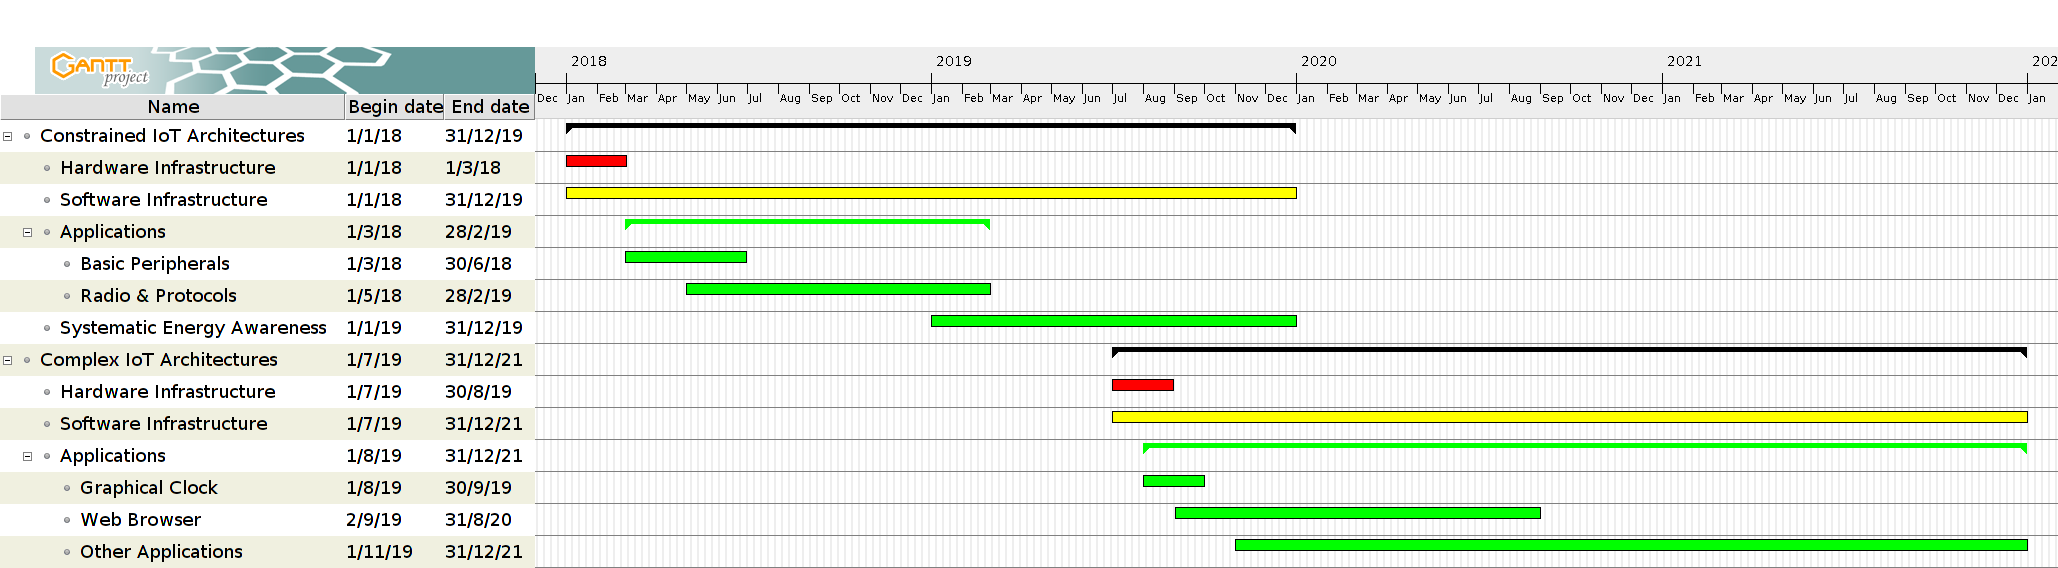
\includegraphics[width=\columnwidth]{serra-big}
    \caption{Cronograma do Projeto
        \label{fig.timeline}
    }
\end{sidewaysfigure}

\newpage
\bibliographystyle{abbrv}
\bibliography{serra}
\end{document}
